\chapter{Exemplos motivacionais}
\label{cap:exemplos}

\textit{Breaking changes} ocorrem de diversas maneiras no ecossistema do \textsf{npm}. Pelo fato do \textsf{Javascript} ser de tipagem dinâmica, o cliente pode ser afetado por muitos erros inesperados, o que finalizará sua execução. Considere os seguintes casos de \textit{breaking changes} que foram detectados nesse trabalho. O primeiro caso ocorre no provedor \textsf{optipng}. Ao atualizar da \textit{release 0.1.1} para \textit{0.2.0}, o provedor introduziu uma alteração no nome de uma de suas \textit{APIs} renomeando \texttt{OptiPng.getBinaryPath} para \texttt{OptiPng.getBinPath},\footnote{https://github.com/papandreou/node-optipng/commit/920216} como no \textit{diff} do Código \ref{cod:diff:optipng}. Após publicar a \textit{release 0.2.0}, todos os clientes que tinham acesso àquela \textit{API} e atualizaram o \textsf{optipng} -- ou receberam a atualização automaticamente devido ao \textit{range} --, passaram a receber um erro de execução pois a \textit{API} prévia não estava mais disponível. Os clientes que utilizavam o \textit{range caret} apenas esperavam receber atualizações retro-compatíveis, mas receberam uma \textit{breaking change}. Um erro de alteração do nome de \textit{APIs} é um erro facilmente detectável, mas a \textit{breaking change} introduzida em \textsf{optipng@0.2.0} foi corrigida depois de 34 dias para a \textit{release 0.3.1}.\footnote{https://github.com/papandreou/node-optipng/commit/a155f2b} No período que essa \textit{breaking change} ficou sem correção, o provedor \textsf{optipng} recebeu \textit{2,8k} \textit{downloads} do \textsf{npm}.

\begin{lstlisting}[numbers=none, language=diff, label=cod:diff:optipng, caption={\textit{Breaking change} de alteração de API no pacote \textsf{optipng}}.]
- OptiPng.getBinaryPath = memoizeAsync(function (cb) {
+ OptiPng.getBinPath = memoizeAsync(function getBinPathAsync(cb) {
\end{lstlisting}

O segundo exemplo de \textit{breaking changes} ocorre no pacote cliente \textsf{ember-cli-chartjs}. A \textit{release 2.1.1} do cliente \textsf{ember-cli-chartjs} especifica dois provedores: \textsf{ember-cli-qunit@\textasciicircum1.2.2} e \textsf{broccoli-asset-rev@\textasciicircum2.4.2}. O provedor \textsf{broccoli-asset-rev} especifica como seu provedor o pacote \textsf{broccoli-filter@\textasciicircum1.2.2}, que por sua vez especifica como seu provedor o pacote \textsf{broccoli-plugin@\textasciicircum1.0.0}. Essa árvore de dependências pode ser visualizada na Figura \ref{fig:dependency_tree}.

\begin{figure}
    \centering
    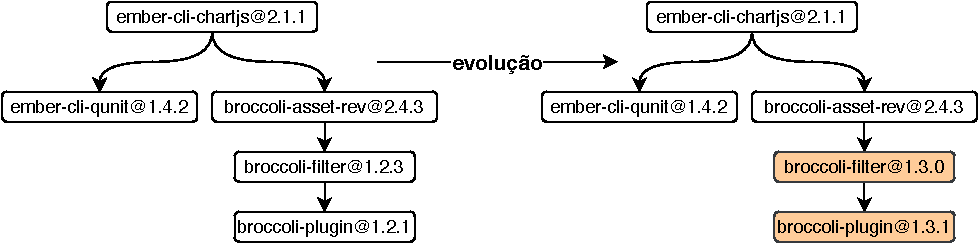
\includegraphics[scale=0.9]{figuras/bc_example_full.pdf}
    \caption{Evolução da árvore de dependências para o pacote cliente \textsf{ember-cli-chartjs} de quando foi publicada a \textit{release 2.1.1} (esquerda) para quando foi executada nesse trabalho (direita).}
    \label{fig:dependency_tree}
\end{figure}

A \textit{release} \textsf{ember-cli-chartjs@2.1.1} foi publicada em Junho de 2016 e executou os testes com sucesso nas determinadas versões de seus provedores até essa data \footnote{https://travis-ci.org/github/busy-web/ember-cli-
chartjs/builds/139575556} (Árvore esquerda da Figura \ref{fig:dependency_tree}). Porém, alguns meses antes, em Novembro de 2015, o provedor \textsf{ember-cli-qunit} publicou a \textit{release 1.0.4} que introduz uma correção de um erro. Essa \textit{release} alterava o tipo de um objeto que era retornado,\footnote{https://github.com/ember-cli/ember-cli-qunit/commit/6fdfe7d} como no diff do Código \ref{cod:bc:ember}, e essa \textit{release} executou com sucesso.

\begin{lstlisting}[numbers=none, language=diff, label=cod:bc:ember, caption={Alteração no tipo do objeto retornado em \textsf{ember-cli-qunit@1.0.4}.}]
 // Skip if useLintTree === false.
 if (this.options['ember-cli-qunit'] && /* ... *\) {
-    return tree;
+    // Fakes an empty broccoli tree
+    return { inputTree: tree, rebuild: function() { return []; } };
 }
\end{lstlisting}

Aproximadamente três anos depois do \textsf{ember-cli-qunit@1.0.4}, em Agosto de 2018, \textsf{broccoli-plugin@1.3.1} foi publicada (Árvore de dependências à direita na Figura \ref{fig:dependency_tree}) e introduziu um alteração em uma função de validação. Essa \textit{release 1.3.1} introduziu uma melhoria na função \texttt{isPossibleNode} para consertar um erro que permitia a validação de objetos inválidos,\footnote{https://github.com/broccolijs/broccoli-plugin/commit/3f9a42b} como no \textit{diff} do Código \ref{cod:bc:ember_2}.

\begin{lstlisting}[numbers=none, language=diff, label=cod:bc:ember_2, caption={broccoli-plugin@1.3.1 validation function enhanced.}]
 function isPossibleNode(node) {
-  return typeof node === 'string' ||
-    (node !== null && typeof node === 'object')
+  var type = typeof node;
+  if (node === null) {
+    return false;
+  } else if (type === 'string') {
   // ...
+  } else {
+    return false;
+  }
}
\end{lstlisting}

Logo que \textsf{broccoli-plugin@1.3.1} foi publicado também foi impactado por uma \textit{breaking change} devido à alteração de objeto de \textsf{ember-cli-qunit@1.0.4},\footnote{https://github.com/broccolijs/broccoli-merge-trees/issues/65} que havia sido publicado quase três anos antes. Essa \textit{breaking change} foi introduzida entre os dois provedores e impactou o pacote cliente, resultando em erros nos seus casos de testes. Então, essa \textit{breaking change} foi consertada em \textsf{ember-cli-qunit@1.4.3} após 15 dias, quando o objeto foi alterado novamente.\footnote{https://github.com/ember-cli/ember-cli-
qunit/commit/59ca6ad} Durante os 15 dias em que a \textit{breaking change} manteve-se não consertada, o pacote \textsf{broccoli-plugin} foi instalado \textit{384k} vezes do \textsf{npm}.

Nesse terceiro exemplo, podemos verificar como que o gerenciamento de dependências pode ser difícil para o pacote cliente. Mesmo quando o cliente se preocupa com as atualizações de seus provedores, alguma \textit{breaking change} pode se manifestar. Por exemplo, o provedor \textsf{jsdom@16} alterou uma de suas funcionalidades para não gerar mais propriedades compartilhadas entre os objetos \footnote{https://github.com/jsdom/jsdom/blob/master/Changelog.md\#1600} -- essa função já havia em versões prévias do \textsf{jsdom}. Quando \textsf{jsdom@16} foi publicado não havia nenhuma incompatibilidade com nenhum de seus provedores. Então, o pacote cliente \textsf{xxx@x.y.z} especificou \textsf{jsdom} como uma versão específica -- talvez para evitar possíveis \textit{breaking changes} nas próximas releases do \textsf{jsdom} --, ou seja, \textsf{xxx} não especifica um \textit{range} de versões para \textsf{jsdom} e os casos de testes executaram com sucesso.

\begin{lstlisting}[numbers=none, language=diff, label=cod:bc:jsdom, caption={\textsf{jsdom@16.3} corrige a função \texttt{installInterface}}]
- exports.installInterfaces = window => {
+ exports.installInterfaces = (window, globalNames) => {
    // Install generated interface.
    for (const generatedInterface of Object.values(generatedInterfaces)) {
-     generatedInterface.install(window);
+     generatedInterface.install(window, globalNames);
  }
\end{lstlisting}

Quase 6 meses depois, foi publicado \textsf{jsdom@16.3} que corrigiu um erro na função do \textsf{jsdom@16}, adicionando um parâmetro que estava faltando quando era executado os seus provedores.\footnote{https://github.com/jsdom/jsdom/commit/e07aac9\#diff-ead812607022ff7c6eca706fca8347ad} O \textit{diff} do Código \ref{cod:bc:jsdom} contém essa correção. Aproximadamente dois meses após da publicação do \textsf{jsdom@16.3}, um dos provedores do \textsf{jsdom}, o pacote \textsf{whatwg-url}, publicou a \textit{release 8.2}, que introduziu uma funcionalidade que é executada pela função \texttt{installInterfaces} do \textsf{jsdom}, a função do Código \ref{cod:bc:jsdom}, e a execução ocorreu com sucesso. Entretanto, o cliente \textsf{xxx} usa o \textsf{jsdom} com um \textit{range} específico e não recebeu a correção publicada em \textsf{jsdom@16.3}. Porém, como \textsf{jsdom@16} especificou o seu provedor, o \textsf{whatwg-url}, com um \textit{range caret}, o cliente \textsf{xxx} recebeu \textsf{whatwg-url@8.2}, que introduziu uma \textit{breaking change} em \textsf{jsdom@16}. O provedor \textsf{whatwg-url@8.2} requer o segundo parâmetro na função \texttt{installInterfaces}, mas esse parâmetro só foi adicionado no \textsf{jsdom@16.3}. Assim, por causa da falta de \textit{range} no cliente e do \textit{range} no \textsf{jsdom}, uma \textit{breaking change}, que foi corrigida oito meses atrás, se manifestou no pacote cliente.